\chapter{Results}
In order to make serious statements about the quality of the code and the effects of using the design patterns some indicators were chosen to compare the two application types. Because the two programs are similar in its work-flow and basic structure these comparisons are actually meaningful. Due to the use git version control bug-fixes do not influence the results.

\section{Lines of Code}
\label{sec:line-count}
In Table \ref{table:lines-of-code} the total lines programmed for both programs and the phases are listed.

\begin{table}
	\centering
	\label{table:lines-of-code}
	\begin{tabular}{|c|c|c|c|c|} \hline
	\textbf{Program version} &\textbf{Phase 1} & \textbf{Phase 2} & \textbf{Phase 3} \\ \hline
	Best practice & 9264 & 12275 & 13306 \\ \hline
	Best practice (adjusted) \footnote{Due to the use of interfaces in java a lot of annotations were necessary which in fact do not have any significance to the topic. Thus the adjusted line count excludes lines that only hold the \texttt{@Override}-Annotation.} & 8804 & 11764 & 12750 \\ \hline
	Ad-hoc & 7572 & 11172 & 12168 \\ \hline
	\end{tabular}
	\caption{Lines of code for both program versions and all phases}
\end{table}

\begin{figure}
	\centering
	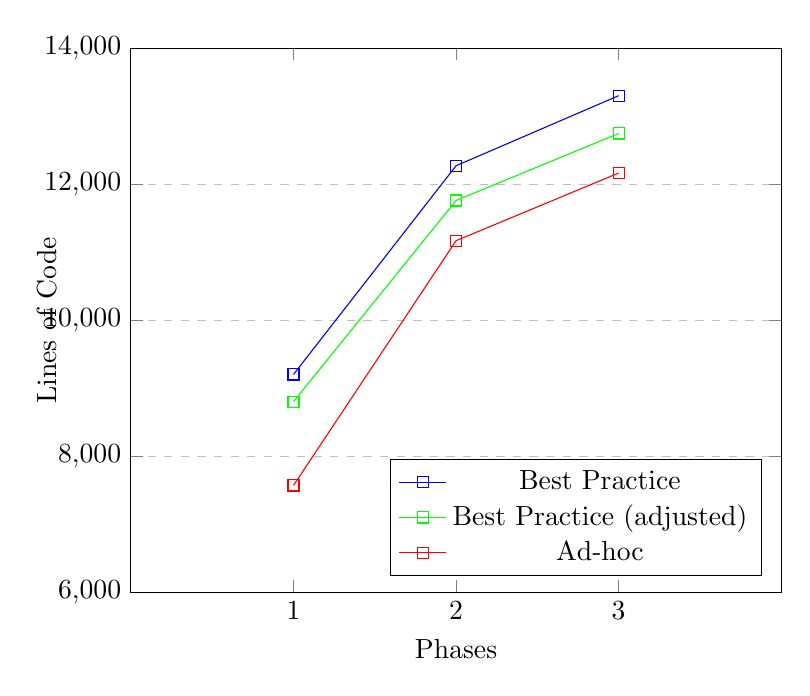
\begin{tikzpicture}
	\begin{axis}[
	height=0.7\textwidth,
	xlabel={Phases},
	ylabel={Lines of Code},
	y label style={at={(axis description cs:-0.1,.5)}},
	xmin=0, xmax=4,
	ymin=6000, ymax=14000,
	xtick={1,2,3},
	ytick={6000, 8000, 10000, 12000, 14000},
	legend pos=south east,
	ymajorgrids=true,
	grid style=dashed,
	scaled ticks=false, 
	tick label style={/pgf/number format/fixed} 
	]
	
	\addplot[
	color=blue,
	mark=square,
	]
	coordinates {
		(1,9205.0)(2,12275.0)(3,13306.0)
	};
	
	\addplot[
	color=green,
	mark=square,
	]
	coordinates {
		(1,8804)(2,11764)(3,12750)
	};

	\addplot[
	color=red,
	mark=square,
	]
	coordinates {
		(1,7572)(2,11172)(3,12168)
	};
	\legend{Best Practice, Best Practice (adjusted), Ad-hoc}
	
	\end{axis}
	
	\end{tikzpicture}
	\caption{Lines of Code for both program versions and all phases}
\end{figure}


\section{Touched and Edited Files}
\label{sec:file-count}
In this section the total number of files and the files that needed to be adopted throughout the phases are compared.

\begin{table}
	\centering
	\label{table:files}
	\begin{tabular}{|c|c|c|c|c|} \hline
		\textbf{Program version} &\textbf{Phase 1} & \textbf{Phase 2} & \textbf{Phase 3} \\ \hline
		Best practice & 96 & 125 & 131 \\ \hline
		Ad-hoc & 59 & 88 & 89 \\ \hline
	\end{tabular}
	\caption{Total number of files for both program versions and all phases}
\end{table}

\begin{figure}
	\centering
	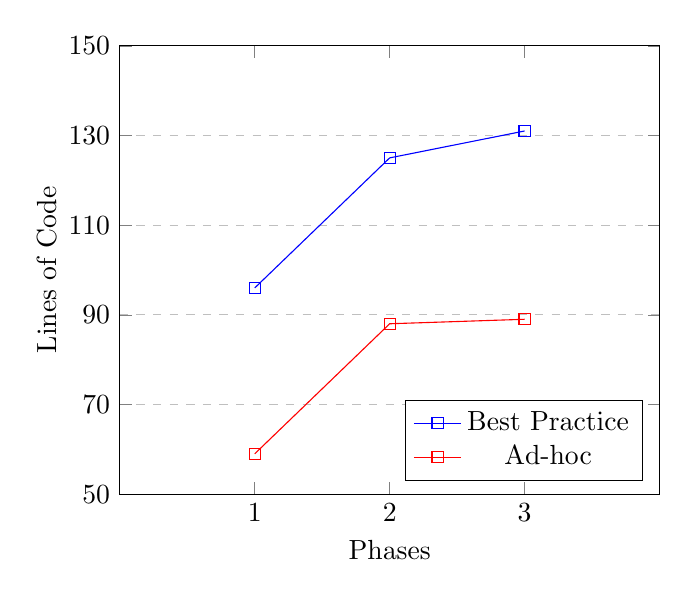
\begin{tikzpicture}
	\begin{axis}[
	xlabel={Phases},
	ylabel={Lines of Code},
	y label style={at={(axis description cs:-0.1,.5)}},
	xmin=0, xmax=4,
	ymin=50, ymax=150,
	xtick={1,2,3},
	ytick={50, 70, 90, 110, 130, 150},
	legend pos=south east,
	ymajorgrids=true,
	grid style=dashed,
	scaled ticks=false, 
	tick label style={/pgf/number format/fixed} 
	]
	
	\addplot[
	color=blue,
	mark=square,
	]
	coordinates {
		(1,96)(2,125)(3,131)
	};
	
	\addplot[
	color=red,
	mark=square,
	]
	coordinates {
		(1,59)(2,88)(3,89)
	};
	\legend{Best Practice, Ad-hoc}
	
	\end{axis}
	
	\end{tikzpicture}
	\caption{Total number of files for both program versions and all phases}
\end{figure}

 \begin{table}
 	\centering
 	\label{table:touched-files}
 	\begin{tabular}{|c|c|c|} \hline
 		\textbf{Program version} &\textbf{Phase 1 to Phase 2} & \textbf{Phase 2 to Phase 3} \\ \hline
 		Best practice & 30 & 7 \\ \hline
 		Ad-hoc & 39 & 13\\ \hline
 	\end{tabular}
 	\caption{Number of files modified or added for both program versions and all phases}
 \end{table}

\section{Average line count per file}
\label{sec:avg-line-count}
Another interesting aspect of the data is the comparison of the average line count per file, as it can be seen in table \ref{table:avg-lines} and chart \ref{fig:avg-lines}. The results are rounded mathematically.

\begin{table}
	\centering
	\label{table:avg-lines}
	\begin{tabular}{|c|c|c|c|} \hline
		\textbf{Program version} &\textbf{Phase 1} & \textbf{Phase 2} & \textbf{Phase 3} \\ \hline
		Best practice & 96 & 98 & 102 \\ \hline
		Best practice (adjusted) & 92 & 94 & 97\\ \hline
		Ad-hoc & 128 & 127 & 137 \\ \hline
	\end{tabular}
	\caption{Average lines per file for both program versions and all phases}
\end{table}

\begin{figure}
	\label{fig:avg-lines}
	\centering
	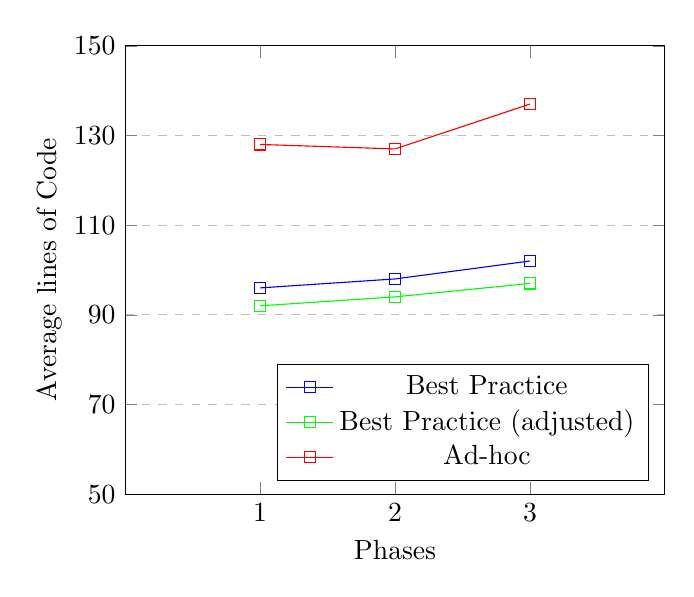
\begin{tikzpicture}
	\begin{axis}[
	xlabel={Phases},
	ylabel={Average lines of Code},
	y label style={at={(axis description cs:-0.1,.5)}},
	xmin=0, xmax=4,
	ymin=50, ymax=150,
	xtick={1,2,3},
	ytick={50, 70, 90, 110, 130, 150},
	legend pos=south east,
	ymajorgrids=true,
	grid style=dashed,
	scaled ticks=false, 
	tick label style={/pgf/number format/fixed} 
	]
	
	\addplot[
	color=blue,
	mark=square,
	]
	coordinates {
		(1,96)(2,98)(3,102)
	};

	\addplot[
	color=green,
	mark=square,
	]
	coordinates {
		(1,92)(2,94)(3,97)
	};
	
	\addplot[
	color=red,
	mark=square,
	]
	coordinates {
		(1,128)(2,127)(3,137)
	};
	\legend{Best Practice, Best Practice (adjusted), Ad-hoc}
	
	\end{axis}
	
	\end{tikzpicture}
	\caption{Total number of files for both program versions and all phases}
\end{figure}
